\newpage
\section*{\textsc{Web Interface Overview}}
\addcontentsline{toc}{section}{Web Interface Overview}
\rhead{\itshape Web Interface Overview}
\lhead{}
\cfoot{\thepage}
\pagestyle{fancy}
\renewcommand{\headrulewidth}{0.4pt}

The ExamGen platform is a responsive web application (light/dark mode) structured
around four sections: \textit{Subjects}, \textit{Archive}, \textit{Exam Builder},
and \textit{Profile}. The screenshots below trace the complete instructor workflow.

\vspace{0.3cm}

%% ── Row 1: Login + Dashboard ────────────────────────────────────────────────
\noindent
\begin{minipage}[t]{0.48\textwidth}
  \centering
  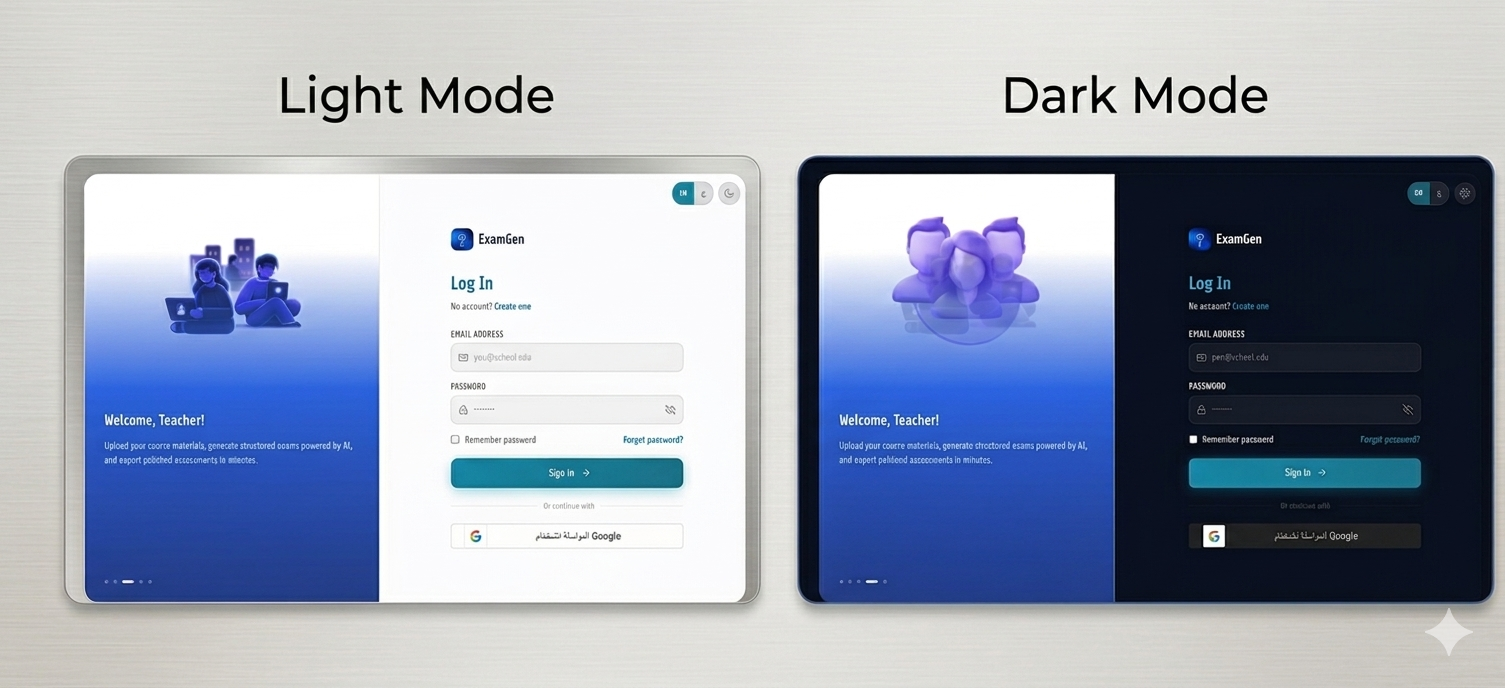
\includegraphics[width=\linewidth]{images/web_login.png}
  \captionof{figure}{Login page (light \& dark mode). Teachers authenticate via
  email/password or Google OAuth~2.0.}
  \label{fig:web_login}
\end{minipage}
\hfill
\begin{minipage}[t]{0.48\textwidth}
  \centering
  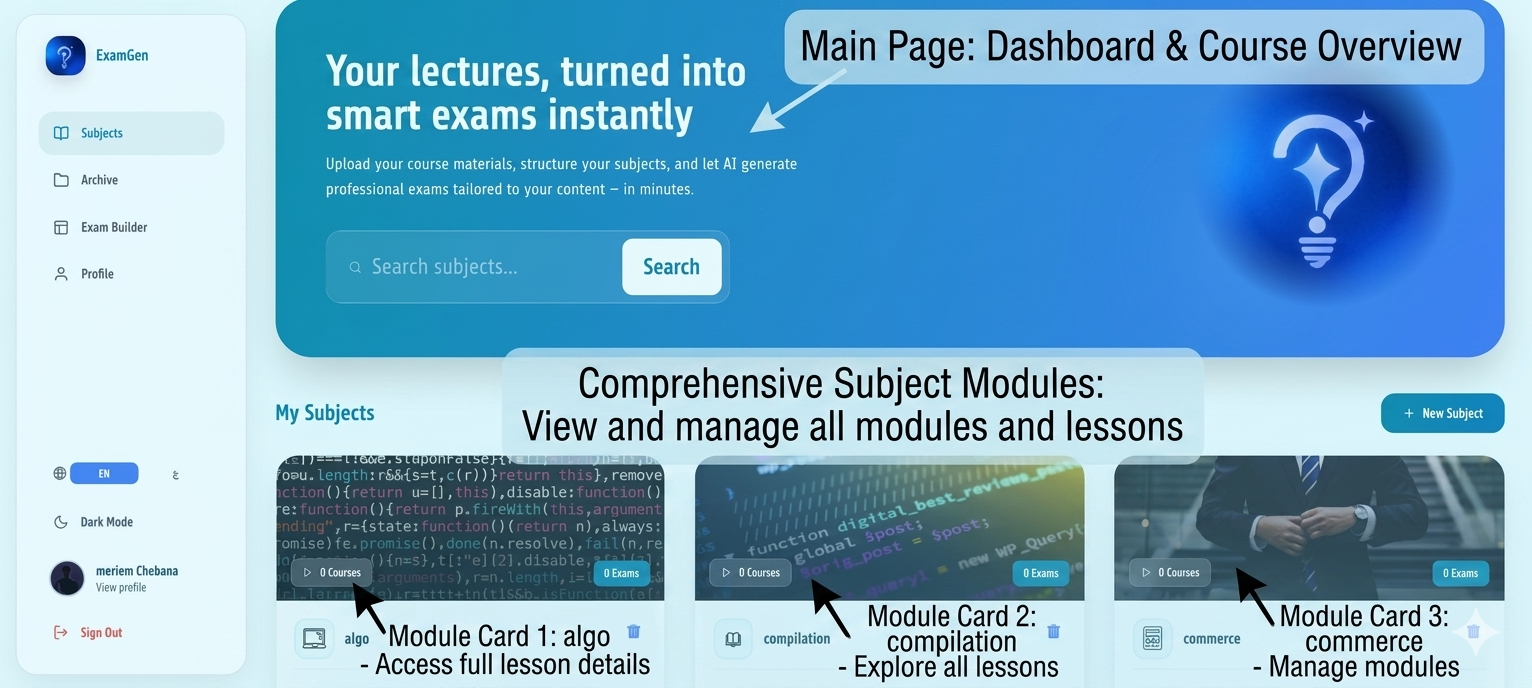
\includegraphics[width=\linewidth]{images/web_dashboard.png}
  \captionof{figure}{Main dashboard: subject cards (Algorithmics, Compilation,
  Commerce\ldots) each grouping courses, exams, and generation history.}
  \label{fig:web_dashboard}
\end{minipage}

\vspace{0.5cm}

%% ── Generation flow (full width) ────────────────────────────────────────────
\begin{center}
  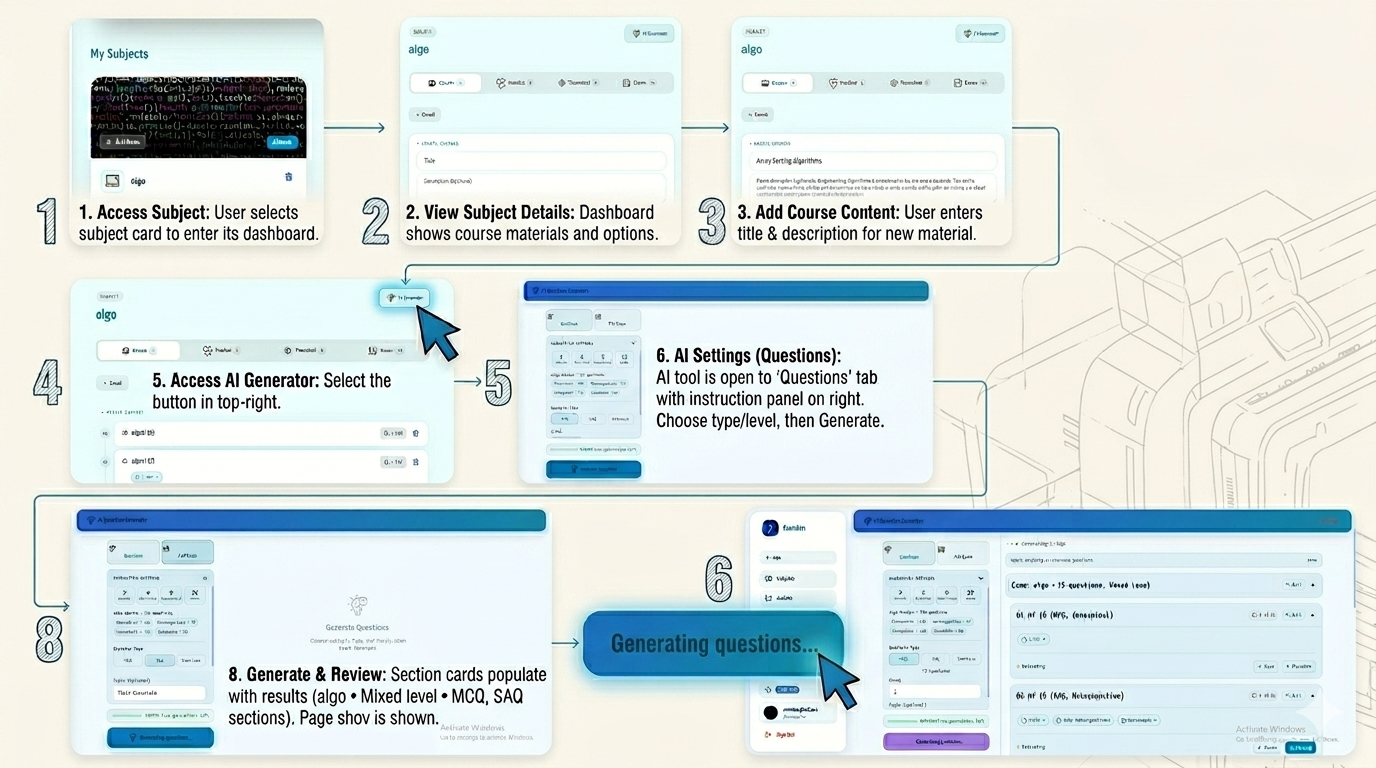
\includegraphics[width=\textwidth, height=6.5cm, keepaspectratio]{images/web_generation.png}
  \captionof{figure}{Exam generation flow: \textbf{(1)}~select subject,
  \textbf{(2)}~view course materials, \textbf{(3)}~add a course,
  \textbf{(5)}~open AI generator, \textbf{(6)}~configure type (MCQ / SAQ / Exercise)
  and Bloom level, \textbf{(7)}~questions stream card-by-card via SSE for
  real-time instructor review.}
  \label{fig:web_generation}
\end{center}

%% ── Row 2: Archive + Builder ────────────────────────────────────────────────
\noindent
\begin{minipage}[t]{0.48\textwidth}
  \centering
  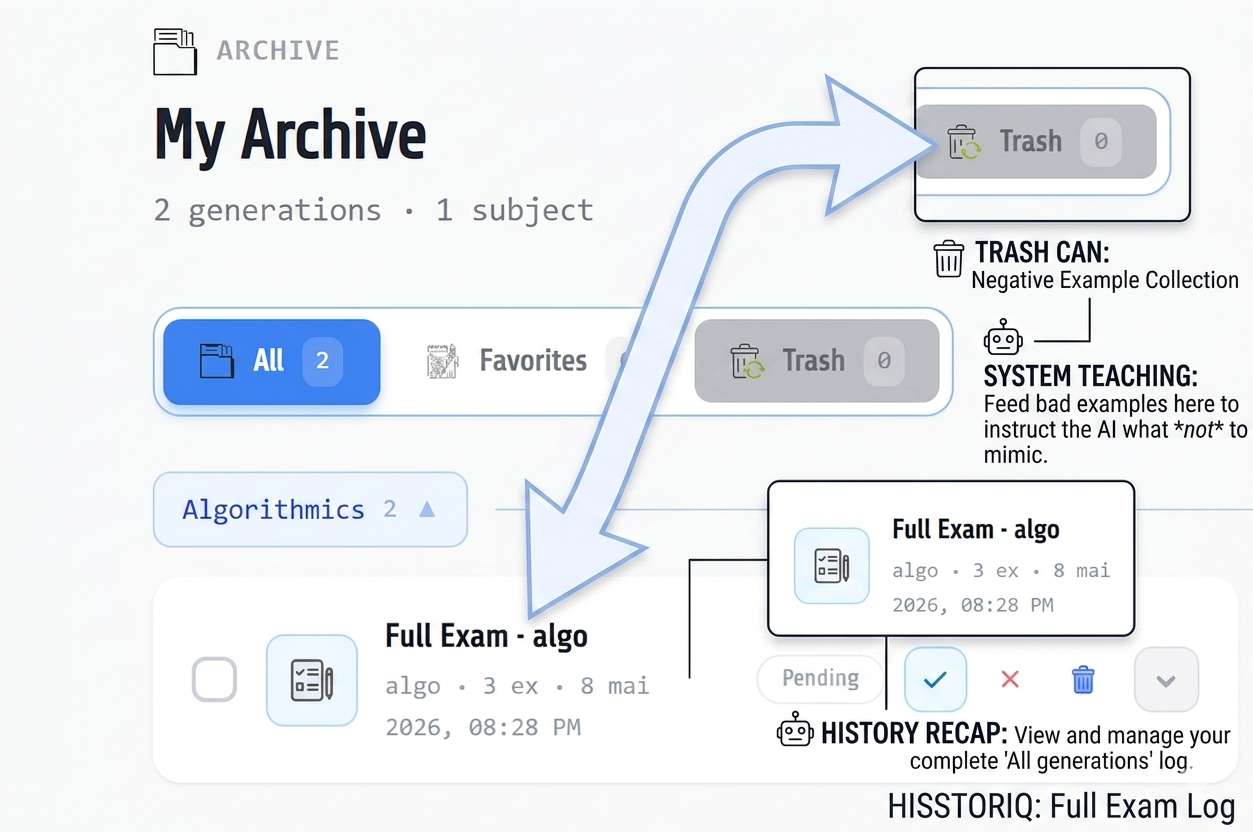
\includegraphics[width=\linewidth]{images/web_archive.png}
  \captionof{figure}{\textbf{Archive \& quality feedback loop.}
  Questions marked as Favorites~($\star$) are validated examples fed back into
  the system as style anchors so that future generations reflect the instructor's
  preferences. Questions sent to Trash are negative examples the system learns
  to avoid.}
  \label{fig:web_archive}
\end{minipage}
\hfill
\begin{minipage}[t]{0.48\textwidth}
  \centering
  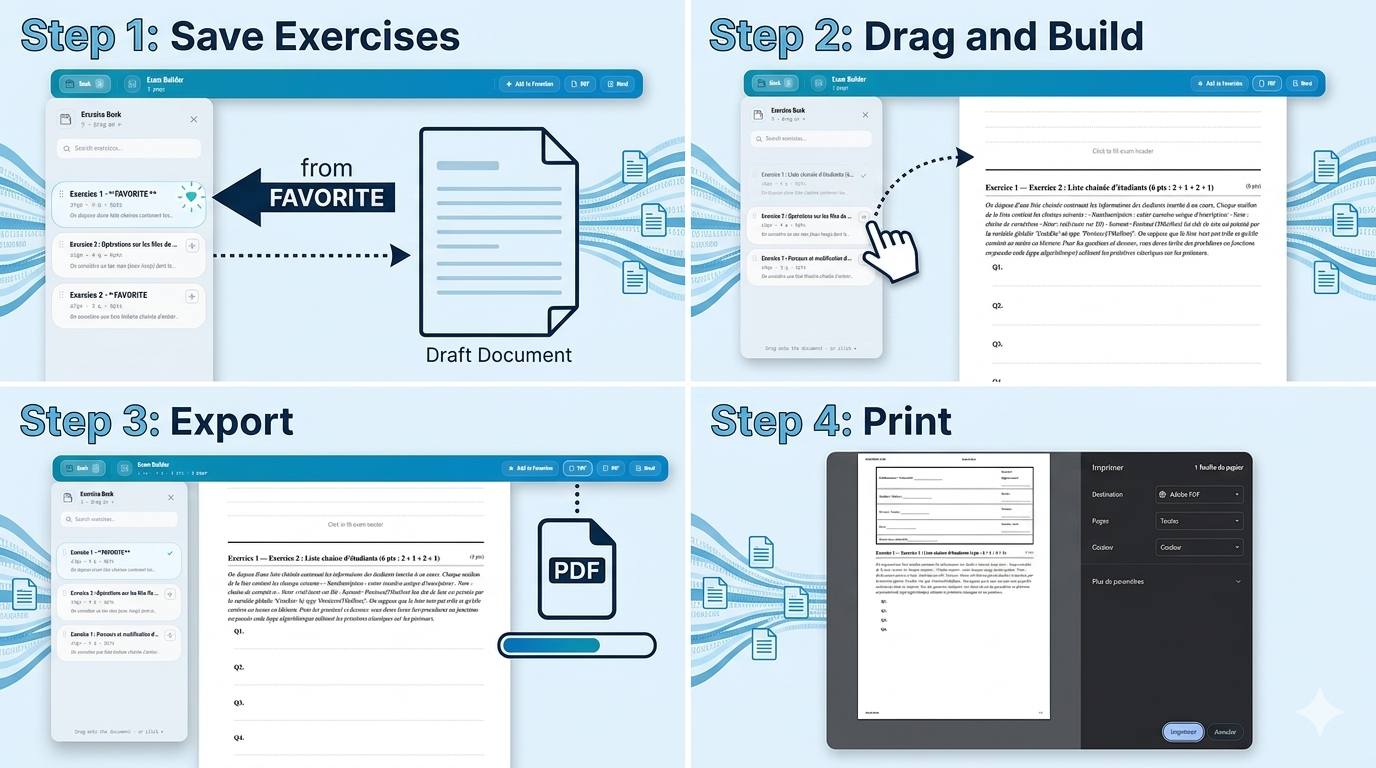
\includegraphics[width=\linewidth]{images/web_builder.png}
  \captionof{figure}{\textbf{Exam Builder (4 steps):}
  save validated exercises from Favorites $\to$ arrange by drag-and-drop $\to$
  export to PDF $\to$ print. The exam header (institution, department, instructor
  name, academic year) is auto-filled from the instructor's \textbf{Profile}.}
  \label{fig:web_builder}
\end{minipage}

\vspace{0.5cm}

%% ── Navigation overview (full width) ────────────────────────────────────────
\begin{center}
  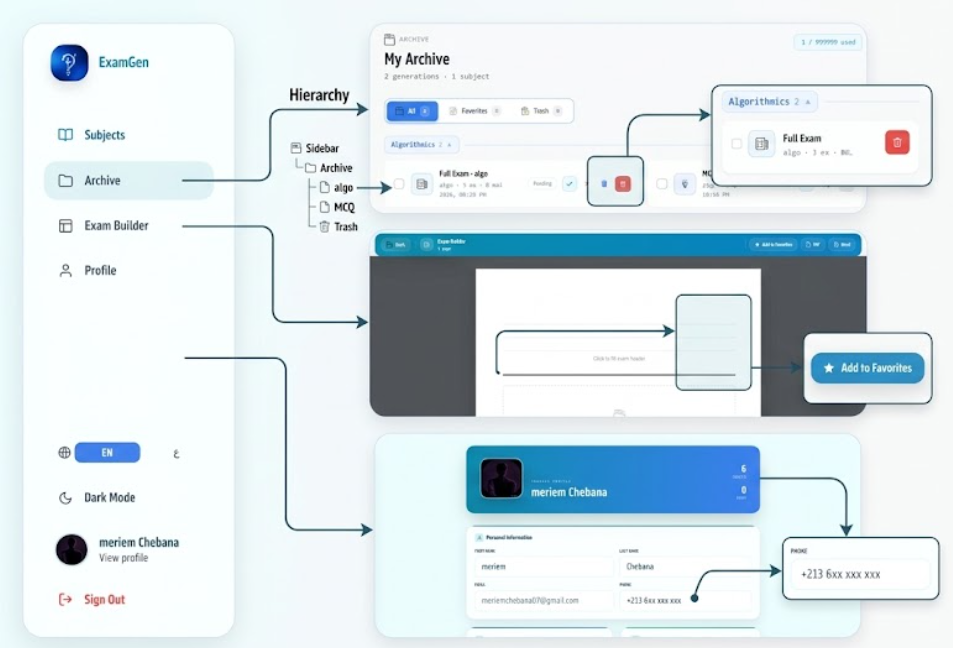
\includegraphics[width=\textwidth, height=5.5cm, keepaspectratio]{images/web_overview.png}
  \captionof{figure}{Full navigation map of the ExamGen application. The persistent
  sidebar links all four sections. The \textbf{Profile} stores institutional
  metadata (university, department, instructor name) injected automatically into
  every exported exam header, ensuring consistent administrative information
  without manual re-entry.}
  \label{fig:web_overview}
\end{center}
